% ===================================================================
%  Week 16 — Persian lecture notes — Transfer Learning & DocScan Capstone
% ===================================================================
\documentclass[12pt,a4paper]{article}
% ===================================================================
%  Shared preamble for Persian lecture notes (Image Processing).
%  Compile with XeLaTeX.  Body = Persian (RTL), code/math = LTR.
% ===================================================================

\usepackage{geometry}
\geometry{a4paper,margin=2.4cm}
\usepackage{amsmath,amssymb}
\usepackage{graphicx}
\usepackage{xcolor}
\usepackage{listings}
\usepackage{tcolorbox}
\usepackage{booktabs}
\usepackage{array}
\usepackage{enumitem}
\usepackage{hyperref}
\tcbuselibrary{skins,breakable}

% ---- Persian / RTL --------------------------------------------------
\usepackage{xepersian}
\settextfont{IRNazli}
\setlatintextfont{Latin Modern Roman}
\setdigitfont{IRNazli}
% More generous leading + paragraph spacing (Persian reads better with air).
\linespread{1.5}
\setlength{\parskip}{0.7em}

% ---- Colours --------------------------------------------------------
\definecolor{coursePrimary}{HTML}{1B4965}
\definecolor{courseAccent}{HTML}{E76F51}
\definecolor{courseGood}{HTML}{2A9D8F}
\definecolor{courseBad}{HTML}{C0392B}
\definecolor{courseInfo}{HTML}{2980B9}
\definecolor{codeBg}{HTML}{F5F6FA}
\definecolor{codeKw}{HTML}{8E44AD}
\definecolor{codeStr}{HTML}{2A9D8F}
\definecolor{codeCom}{HTML}{7F8C8D}

\hypersetup{colorlinks=true,linkcolor=courseInfo,urlcolor=courseInfo,citecolor=courseInfo}

% ---- Code listings (Python built in) -------------------------------
\lstdefinestyle{course}{
  backgroundcolor=\color{codeBg},
  basicstyle=\ttfamily\small,
  keywordstyle=\color{codeKw}\bfseries,
  stringstyle=\color{codeStr},
  commentstyle=\color{codeCom}\itshape,
  numberstyle=\tiny\color{codeCom},
  numbers=left, numbersep=7pt,
  showstringspaces=false, breaklines=true,
  tabsize=4, columns=fullflexible, frame=single,
  rulecolor=\color{gray!30}, keepspaces=true, upquote=true, language=Python,
}
\lstset{style=course}
\lstdefinelanguage{bash}{
  keywords={cd,pip,python,venv,source,import}, sensitive=true,
  morecomment=[l]{\#}, morestring=[b]', morestring=[b]",
}
\newenvironment{ltrcode}{\begin{LTR}}{\end{LTR}}

% ---- Callout boxes (Persian titles) --------------------------------
\newtcolorbox{yaddasht}{colback=courseInfo!8,colframe=courseInfo,
  title={\textbf{یادداشت}},boxrule=0.6pt,right=6pt,left=6pt,breakable}
\newtcolorbox{nokte}{colback=courseAccent!10,colframe=courseAccent,
  title={\textbf{نکتهٔ کلیدی}},boxrule=0.6pt,right=6pt,left=6pt,breakable}
\newtcolorbox{hoshdar}{colback=courseBad!8,colframe=courseBad,
  title={\textbf{هشدار / دام}},boxrule=0.6pt,right=6pt,left=6pt,breakable}
\newtcolorbox{riyazi}{colback=coursePrimary!6,colframe=coursePrimary,
  title={\textbf{ریاضیات}},boxrule=0.6pt,right=6pt,left=6pt,breakable}
\newtcolorbox{tamrin}{colback=courseGood!8,colframe=courseGood,
  title={\textbf{تمرین}},boxrule=0.6pt,right=6pt,left=6pt,breakable}

% ---- Header helper --------------------------------------------------
\newcommand{\coursemeta}[2]{%
  \begin{center}
  {\large\textbf{پردازش تصویرِ کاربردی}}\\[2pt]
  {\color{coursePrimary}\rule{\linewidth}{1pt}}\\[4pt]
  {\Large\textbf{#1}}\\[3pt]
  {\small جزوهٔ درس — #2}
  \end{center}\vspace{4pt}
}


\begin{document}
\coursemeta{جلسهٔ ۱۶ — یادگیریِ انتقالی و پروژهٔ نهاییِ DocScan (Transfer Learning)}{هفتهٔ شانزدهم — پایانی}

\section*{نگاهِ کلی به این جلسه}

به جلسهٔ پایانیِ درس رسیدیم. مسیرِ ما یک قوسِ کامل داشت: در هفتهٔ ۱۲ دیدیم که ویژگی‌های دست‌طراحی (HOG) روی خودروهای شبیه‌به‌هم روی دقتِ \textbf{۰٫۴۸} متوقف شدند؛ در هفتهٔ ۱۳ فهمیدیم CNNها ویژگی‌ها را خودشان یاد می‌گیرند اما به دادهٔ زیاد نیاز دارند. امروز گرهِ ماجرا باز می‌شود: با \textbf{یادگیریِ انتقالی} (transfer learning) از شبکه‌ای که قبلاً روی میلیون‌ها تصویر آموزش دیده استفاده می‌کنیم و — روی \emph{همان} داده و با \emph{همان} طبقه‌بند — دقت را از ۰٫۴۸ به \textbf{۰٫۸۷} می‌رسانیم. سپس کلِ خط‌لولهٔ \textbf{DocScan} را که هر هفته یک تکه‌اش را ساختیم، سرِ‌هم می‌کنیم.

\begin{yaddasht}
پیامِ محوریِ امروز: در بیشترِ پروژه‌های واقعی داده \emph{کم} است. یادگیریِ انتقالی همان چیزی است که به شما اجازه می‌دهد با داده‌ی کم هم از قدرتِ یادگیریِ عمیق بهره ببرید. این، پرکاربردترین تکنیکِ عملیِ یادگیریِ عمیق است.
\end{yaddasht}

\subsection*{یک تشبیهِ ساده}

تصور کنید می‌خواهید زبانِ ایتالیایی یاد بگیرید. دو نفر را در نظر بگیرید: یکی که هیچ زبانی جز فارسی نمی‌داند، و دیگری که پیش‌تر اسپانیایی آموخته است. نفرِ دوم بسیار سریع‌تر یاد می‌گیرد، چون بسیاری از ساختارها، ریشه‌ها و مفاهیم را از اسپانیایی به ایتالیایی \emph{منتقل} می‌کند. لازم نیست او از صفر شروع کند. یادگیریِ انتقالی دقیقاً همین است: شبکه‌ای که «زبانِ دیدن» را روی میلیون‌ها تصویرِ ImageNet آموخته، بیشترِ آن دانش را به تسکِ جدیدِ شما (تشخیصِ خودرو یا خواندنِ کنتور) منتقل می‌کند و فقط باید «واژگانِ» تخصصیِ تسکِ شما را یاد بگیرد. به همین دلیل با دادهٔ کم و آموزشِ کوتاه به نتیجهٔ خوب می‌رسیم.

\section{مسئلهٔ دادهٔ کم}

چرا نمی‌توانیم صرفاً یک CNNِ بزرگ روی داده‌های خودمان آموزش دهیم؟ چون CNNهای عمیق میلیون‌ها پارامتر دارند و برای برازشِ بدونِ بیش‌برازش به $۱۰^۴$ تا $۱۰^۶$ تصویرِ برچسب‌دار نیاز دارند. ما فقط ۶۰ تصویر در هر مدلِ خودرو داریم؛ آموزشِ یک شبکهٔ بزرگ از صفر روی این داده به‌شدت بیش‌برازش می‌کند و روی آزمون فرو می‌ریزد.

از سوی دیگر، سقفِ ۰٫۴۸ ویژگیِ دستی نشان داد که HOG هم کافی نیست. پس در یک بن‌بست به‌نظر می‌رسیم: نه دادهٔ کافی برای یادگیریِ عمیق داریم، نه ویژگیِ دستیِ قدرتمند.

\begin{nokte}
راهِ خروج از این بن‌بست، مشاهده‌ای ظریف است: لازم نیست ویژگی‌ها را \emph{ما} یاد بگیریم و لازم هم نیست از \emph{صفر} یادشان بگیریم. می‌توانیم ویژگی‌هایی را که یک شبکهٔ دیگر روی دادهٔ عظیم یاد گرفته «قرض» بگیریم.
\end{nokte}

\section{بینشِ کلیدیِ یادگیریِ انتقالی}

یک CNN که روی ImageNet (۱٫۲ میلیون تصویر، ۱۰۰۰ کلاس) آموزش دیده، ویژگی‌های بصریِ \emph{عمومی} یاد گرفته است: لبه‌ها، بافت‌ها، شکل‌ها، اجزا. نکتهٔ حیاتی این است که این ویژگی‌های اولیه و میانی برای \emph{تقریباً هر} تسکِ تصویری مفیدند — از جمله تشخیصِ مدلِ خودرو.

\begin{yaddasht}
پس ایدهٔ یادگیریِ انتقالی ساده است: به‌جای یادگرفتنِ ویژگی‌ها از صفر، آن‌ها را از یک شبکهٔ از‌پیش‌آموخته \emph{بازاستفاده} کنیم. لایه‌های نخستِ یک شبکهٔ بیناییِ خوب، یک «استخراج‌گرِ ویژگیِ همه‌منظوره» است؛ هدر‌دادنش عاقلانه نیست.
\end{yaddasht}

\subsection{دو شیوهٔ یادگیریِ انتقالی}

\begin{center}
\begin{tabular}{@{}lll@{}}
\hline
\textbf{شیوه} & \textbf{چه می‌کنید} & \textbf{کِی} \\
\hline
استخراجِ ویژگی & شبکه را منجمد کن، فقط یک سرِ طبقه‌بندِ نو آموزش بده & دادهٔ خیلی کم \\
تنظیمِ دقیق (fine-tune) & برخی لایه‌های بالا را باز کن و آموزش بده & دادهٔ بیشتر \\
\hline
\end{tabular}
\end{center}

ما از \textbf{استخراجِ ویژگی} استفاده کردیم: یک شبکهٔ ConvNeXtِ منجمدِ آموخته‌شده‌روی‌ImageNet هر خودرو را به یک بردارِ ۱۰۲۴‌بُعدی تبدیل می‌کند، و سپس یک SVM طبقه‌بندی می‌کند — دقیقاً همان طبقه‌بندِ هفتهٔ ۱۲، فقط با ویژگی‌های بهتر.

\section{نتیجهٔ ما: سقف بالا می‌رود}

نتیجهٔ واقعیِ اجرا روی همان مسئلهٔ ۲۰۶/۴۰۵/دنا:

\begin{center}
  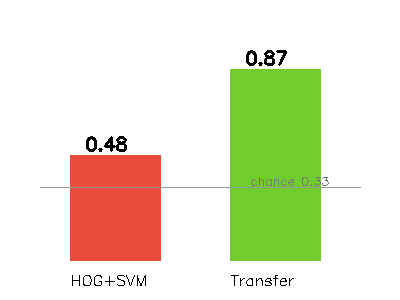
\includegraphics[width=0.4\linewidth]{../assets/accuracy_bars.png}\hfill
  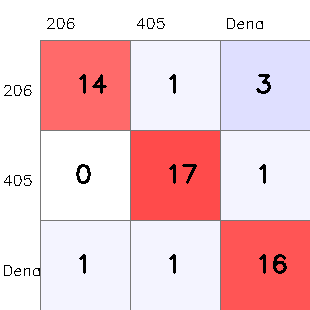
\includegraphics[width=0.34\linewidth]{../assets/confusion_transfer.png}\\
  {\small چپ: مقایسهٔ دقت (HOG+SVM ۰٫۴۸ در برابرِ انتقالی ۰٫۸۷) \quad راست: ماتریسِ درهم‌ریختگیِ انتقالی}
\end{center}

دقت کنید که چه چیزی \emph{تغییر نکرد}: همان ۱۸۰ تصویر، همان SVM، همان تقسیمِ آموزش/آزمون. تنها تغییر: HOG جای خود را به ویژگی‌های منجمدِ ImageNet داد. نتیجه: \textbf{۰٫۴۸ به ۰٫۸۷}. یعنی ویژگی‌ها از همان ابتدا گلوگاه بودند، نه طبقه‌بند.

\begin{nokte}
ماتریسِ درهم‌ریختگیِ سمتِ راست حالا قطرِ غالب دارد (بیشترِ خودروها درست طبقه‌بندی شده‌اند)، در مقابلِ ماتریسِ تقریباً‌تصادفیِ هفتهٔ ۱۲. شبکهٔ از‌پیش‌آموخته تفاوت‌های ظریفی را «می‌بیند» که HOG از دست می‌داد — مثلِ شکلِ جلوپنجره و الگوی چراغ‌ها.
\end{nokte}

\subsection{چرا ۱۰۲۴ بُعد بهتر از ۹۰۰ بُعدِ HOG است؟}

شاید بپرسید فرقِ بردارِ ۱۰۲۴‌بُعدیِ عمیق با بردارِ ۹۰۰‌بُعدیِ HOG در چیست — هر دو که فقط عدد‌اند. تفاوت در \emph{معنای} این اعداد است.

\begin{riyazi}
هر عددِ HOG می‌گوید «در این سلول، چقدر لبه در این جهت هست» — یک ویژگیِ سطحِ‌پایین و ثابت. اما هر عددِ بردارِ عمیق، خروجیِ یک آشکارسازِ آموخته‌شده روی میلیون‌ها تصویر است و می‌تواند مفاهیمِ سطحِ‌بالا را کد کند: «چقدر شبیهِ جلوپنجرهٔ مشبک است»، «چقدر الگوی چراغِ کشیده دارد». این ویژگی‌های \emph{معنایی}، کلاس‌ها را در فضای ۱۰۲۴‌بُعدی بسیار جداپذیرتر می‌کنند.
\end{riyazi}

\begin{yaddasht}
به عبارتِ دیگر، بُعد‌ها مهم نیستند، \emph{کیفیتِ} بُعد‌ها مهم است. ۱۰۲۴ عددِ معنادار از یک شبکهٔ آموخته، بسیار ارزشمندتر از ۹۰۰ عددِ سطحِ‌پایینِ دستی است. همین، جهشِ ۰٫۴۸ به ۰٫۸۷ را توضیح می‌دهد.
\end{yaddasht}

\subsection{چرا این‌قدر خوب کار می‌کند؟}

\begin{itemize}
  \item ImageNet شاملِ خودروهای فراوان است، پس شبکه از قبل اجزای مرتبط با خودرو را یاد گرفته.
  \item ویژگی‌های سطحِ‌میانیِ آن (شکلِ جلوپنجره، الگوی چراغ) دقیقاً همان چیزی است که مدل‌ها را از هم جدا می‌کند.
  \item قدرتِ یک شبکهٔ عظیم را با فقط ۶۰ تصویر در هر کلاس و چند ثانیه آموزش به دست می‌آوریم.
\end{itemize}

\subsection{کدامَ لایه چه چیزی منتقل می‌کند؟}

همهٔ لایه‌های یک شبکه به یک اندازه قابلِ انتقال نیستند:

\begin{itemize}
  \item \textbf{لایه‌های اولیه:} لبه‌ها، رنگ‌ها، بافت‌ها — جهانی‌اند و به \emph{هر} تسکی منتقل می‌شوند.
  \item \textbf{لایه‌های میانی:} اجزا و نقش‌مایه‌ها — به دامنه‌های مرتبط خوب منتقل می‌شوند.
  \item \textbf{لایه‌های پایانی:} مخصوصِ کلاس‌اند (مثلاً «سگِ نژادِ خاص») — کمترین قابلیتِ انتقال؛ اغلب جایگزین می‌شوند.
\end{itemize}

\begin{riyazi}
قاعدهٔ سرانگشتی: هرچه تسکِ شما از ImageNet متفاوت‌تر باشد، باید لایه‌های پایانیِ بیشتری را دوباره آموزش دهید. برای عکس‌های معمولی (خودرو، کنتور) که «فاصلهٔ دامنه» (domain gap) کوچک است، انجمادِ کامل + استخراجِ ویژگی کافی است — و همین ۰٫۸۷ ما را داد.
\end{riyazi}

\subsection{تنظیمِ دقیق (fine-tuning) چطور کار می‌کند؟}

اگر دادهٔ بیشتری داشتید و استخراجِ ویژگیِ ساده کافی نبود، گامِ بعدی تنظیمِ دقیق است:

\begin{enumerate}
  \item از وزن‌های از‌پیش‌آموخته شروع کن (نه از وزن‌های تصادفی).
  \item لایهٔ طبقه‌بندیِ آخر را با یک لایهٔ نو برای تعدادِ کلاس‌های خودت جایگزین کن.
  \item لایه‌های اولیه را منجمد نگه دار و فقط لایه‌های بالایی را با \emph{نرخِ یادگیریِ کوچک} آموزش بده.
\end{enumerate}

\begin{hoshdar}
نرخِ یادگیری در تنظیمِ دقیق باید کوچک باشد (مثلاً ۱۰ تا ۱۰۰ برابر کوچک‌تر از آموزش از صفر). وگرنه گام‌های بزرگ، دانشِ باارزشِ از‌پیش‌آموخته را «فراموش» می‌کنند — پدیده‌ای به نامِ «فراموشیِ فاجعه‌بار» (catastrophic forgetting).
\end{hoshdar}

\subsection{افزایشِ داده برای دادهٔ کم}

یک هم‌دستِ عالی برای یادگیریِ انتقالی، \textbf{افزایشِ داده} (data augmentation) است: داده را رایگان چند‌برابر کنید با چرخش‌های کوچک، وارونه‌سازیِ افقی، تغییرِ روشنایی/کنتراست و برش‌های تصادفی. هر گونه، همان برچسب را زیرِ یک تغییرِ بی‌اهمیتِ جدید به شبکه می‌آموزد و در نتیجه ناوردایی بیشتر و بیش‌برازشِ کمتر می‌دهد.

\begin{nokte}
افزایشِ داده ارزان‌ترین دقتی است که می‌خرید؛ روی مسائلِ دادهٔ کم همیشه امتحانش کنید. اما مراقب باشید: افزایشی که برچسب را عوض کند بد است — مثلاً وارونه‌سازیِ عمودیِ یک رقم، ۶ را به ۹ تبدیل می‌کند!
\end{nokte}

\section{خط‌لولهٔ کاملِ DocScan}

حالا به هدفِ نهاییِ درس می‌رسیم: سرِ‌هم‌کردنِ کلِ سامانهٔ DocScan که هر هفته یک مهرهٔ آن را ساختیم. شکلِ زیر خط‌لوله را روی یک نوارِ ارقامِ کنتورِ واقعی نشان می‌دهد:

\begin{center}
  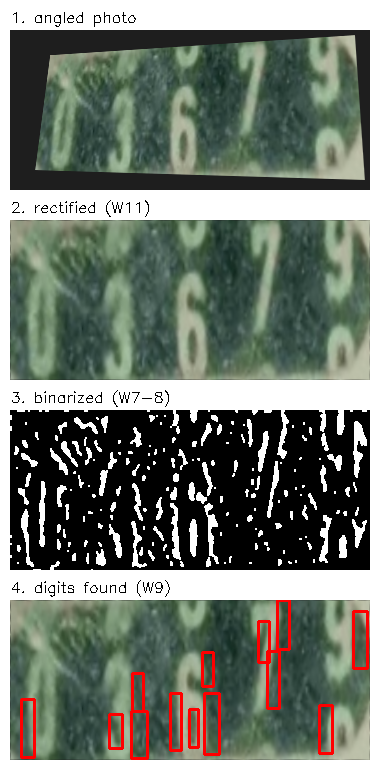
\includegraphics[height=0.55\textheight]{../assets/docscan_pipeline.png}\\
  {\small پنج مرحله: عکسِ کج $\rightarrow$ صاف‌سازی $\rightarrow$ باینری‌سازی $\rightarrow$ جداسازیِ ارقام $\rightarrow$ خواندن}
\end{center}

\begin{enumerate}
  \item \textbf{عکس:} کنتوری که از زاویه عکس گرفته شده (ورودیِ خام).
  \item \textbf{صاف‌سازی (هفتهٔ ۱۱):} هوموگرافی عکس را به نمای روبه‌رو تبدیل می‌کند.
  \item \textbf{باینری‌سازی (هفته‌های ۲/۷/۸):} آستانه + مورفولوژی تصویر را تمیز می‌کند.
  \item \textbf{جداسازی (هفتهٔ ۹):} کانتورها کادرِ هر رقم را پیدا می‌کنند.
  \item \textbf{خواندن (هفتهٔ ۱۳):} یک CNN هر رقم را طبقه‌بندی می‌کند $\rightarrow$ «۰۳۶۷۹».
\end{enumerate}

\subsection{هر هفته یک مرحله بود}

\begin{center}
\begin{tabular}{@{}ll@{}}
\hline
\textbf{هفته‌ها} & \textbf{نقش در DocScan} \\
\hline
۱ تا ۴: پیکسل، هیستوگرام، فیلتر، حذفِ نویز & تمیزکردنِ عکسِ خام \\
۵ تا ۶: لبه، فوریه & یافتنِ ساختار، حذفِ نویزِ تناوبی \\
۷ تا ۹: مورفولوژی، بخش‌بندی، کانتور & جداکردنِ ارقام \\
۱۰ تا ۱۱: ویژگی، هوموگرافی & صاف‌سازی به اسکنِ تخت \\
۱۲ تا ۱۶: یادگیریِ ماشین، CNN، انتقالی & خواندنِ ارقام \\
\hline
\end{tabular}
\end{center}

\begin{yaddasht}
DocScan یک پروژهٔ جدا نبود؛ ستونِ فقراتی بود که هر هفته یک مهره به آن اضافه کردیم. همین نشان می‌دهد که یک سامانهٔ واقعیِ بینایی، زنجیره‌ای از تکنیک‌هاست، نه یک تکنیکِ واحد.
\end{yaddasht}

\section{کدِ یادگیریِ انتقالی}

\begin{ltrcode}
\begin{lstlisting}[language=Python]
import torch, torch.nn as nn
from torchvision.models import convnext_base, ConvNeXt_Base_Weights
from sklearn.svm import SVC

weights = ConvNeXt_Base_Weights.IMAGENET1K_V1
model = convnext_base(weights=weights).eval()      # pretrained
feat = nn.Sequential(model.features, model.avgpool, nn.Flatten())
pre = weights.transforms()          # use the model's OWN preprocessing!

def embed(bgr):                     # image -> 1024-D deep feature
    rgb = cv2.cvtColor(bgr, cv2.COLOR_BGR2RGB)
    t = pre(torch.tensor(rgb).permute(2,0,1)).unsqueeze(0)
    with torch.no_grad():
        return feat(t).numpy().ravel()

X = [embed(img) for img in images]  # deep features, not HOG
clf = SVC(kernel='rbf', C=10).fit(Xtr, ytr)   # same SVM as Week 12
\end{lstlisting}
\end{ltrcode}

\begin{hoshdar}
مهم‌ترین خطِ این کد \texttt{pre = weights.transforms()} است. هر شبکهٔ از‌پیش‌آموخته انتظارِ پیش‌پردازشِ خاصِ خود را دارد (اندازهٔ ورودی، میانگین/انحرافِ‌معیارِ نرمال‌سازی). اگر پیش‌پردازشِ اشتباه بدهید، ویژگی‌ها بی‌معنی می‌شوند و دقت فرو می‌ریزد. همیشه از پیش‌پردازشِ رسمیِ خودِ مدل استفاده کنید.
\end{hoshdar}

\section{اشتباه‌های رایج در یادگیریِ انتقالی}

\begin{itemize}
  \item \textbf{پیش‌پردازشِ ناهماهنگ:} همان‌طور که گفتیم، رایج‌ترین و مخرب‌ترین اشتباه.
  \item \textbf{فراموشیِ حالتِ eval:} اگر \texttt{model.eval()} را فراموش کنید، لایه‌های BatchNorm/Dropout در حالتِ آموزش می‌مانند و ویژگی‌ها ناپایدار می‌شوند.
  \item \textbf{نرمال‌نکردنِ ویژگی‌ها پیش از SVM:} ویژگی‌های عمیق مقیاس‌های متفاوت دارند؛ استانداردسازی اغلب کمک می‌کند.
  \item \textbf{تنظیمِ دقیق با نرخِ یادگیریِ بزرگ:} دانشِ از‌پیش‌آموخته را نابود می‌کند.
  \item \textbf{نشتِ داده:} استخراجِ ویژگی روی کلِ داده پیش از تقسیم، سپس تقسیم — همان دامِ هفتهٔ ۱۲.
\end{itemize}

\begin{nokte}
جالب است که بیشترِ این اشتباه‌ها دربارهٔ \emph{مدل} نیستند، بلکه دربارهٔ \emph{داده و پیش‌پردازش}‌اند. این یک درسِ تکرارشوندهٔ کلِ بخشِ یادگیری است: کیفیتِ داده و درستیِ خط‌لوله، بیش از انتخابِ مدل اهمیت دارد.
\end{nokte}

\section{مهندسیِ یک خط‌لولهٔ مقاوم}

تفاوتِ یک «دمو» و یک «محصول» در مدیریتِ شکست است. یک دمو روی یک عکسِ تمیز کار می‌کند؛ یک محصول باید در برابرِ تاری، انعکاسِ نور، کجی و کثیفی دوام بیاورد.

\begin{itemize}
  \item \textbf{دروازه‌های اطمینان (confidence gates):} اگر تعدادِ درون‌داده‌های RANSAC کم بود، به‌جای حدس‌زدن، عکسِ جدید بخواه.
  \item \textbf{بررسیِ سلامت (sanity checks):} خوانشِ کنتور تعدادِ ثابتی رقم دارد؛ خوانشِ با تعدادِ اشتباه را رد کن.
  \item \textbf{مسیرهای جایگزین (fallbacks):} اگر مسیرِ ویژگی شکست خورد، مسیرِ کانتور را امتحان کن و برعکس.
  \item \textbf{ثبتِ لاگ (logging):} کیفیتِ هر مرحله (خطای بازتصویر، اطمینانِ ارقام) را ثبت کن تا بتوانی شکست‌ها را عیب‌یابی کنی.
\end{itemize}

\begin{hoshdar}
همیشه «برای شکست طراحی کنید». پرسشِ درست این نیست «آیا روی این عکس کار می‌کند؟» بلکه «وقتی عکسِ بد بیاید، سامانه چه می‌کند؟». پاسخِ خوب، رد‌کردنِ مؤدبانه و درخواستِ ورودیِ بهتر است، نه تولیدِ خروجیِ غلطِ بی‌سر‌و‌صدا.
\end{hoshdar}

\section{صداقت، اخلاق و محدودیت‌ها}

\begin{itemize}
  \item عددِ \emph{آزمون}، موارِد شکست، و داده‌ای که روی آن آموزش دیده‌اید را گزارش کنید — نه فقط بهترین دمو.
  \item یک رقمِ کنتورِ اشتباه یعنی یک قبضِ اشتباه؛ نرخِ خطایتان را بدانید و خوانش‌های کم‌اطمینان را دروازه‌بندی کنید.
  \item مراقبِ سوگیریِ داده باشید: اگر همهٔ کنتورهای آموزشی تمیز و روشن باشند، انتظارِ شکست روی کنتورهای کثیف را داشته باشید.
\end{itemize}

\begin{nokte}
«۹۷٪ دقیق» بدونِ این سه چیز بی‌معنی است: روی چه داده‌ای، با کدام سنجه، و چطور شکست می‌خورد. یک مهندسِ خوب همیشه این سه را کنارِ هر عدد گزارش می‌کند.
\end{nokte}

\section{قوسِ کاملِ درس}

از یک تک‌پیکسل آغاز کردیم و به یک شبکهٔ عصبیِ از‌پیش‌آموخته رسیدیم. دو نیمهٔ درس مکملِ هم‌اند:

\begin{itemize}
  \item \textbf{پردازش تصویرِ کلاسیک (هفته‌های ۱ تا ۱۱):} دقیق، قابلِ‌تفسیر، بدونِ نیاز به آموزش — هنوز برای هندسه و پاک‌سازی ضروری است.
  \item \textbf{یادگیری (هفته‌های ۱۲ تا ۱۶):} قدرتمند برای شناسایی، به‌ویژه با یادگیریِ انتقالی.
  \item \textbf{یک سامانهٔ واقعی از هر دو استفاده می‌کند:} کلاسیک برای آماده‌سازی، آموخته برای شناسایی.
\end{itemize}

\subsection{مرورِ کاملِ ۱۶ هفته}

\begin{center}
\begin{tabular}{@{}cll@{}}
\hline
\textbf{هفته} & \textbf{موضوع} & \textbf{مهارتِ کلیدی} \\
\hline
۱ & پیکسل‌ها و هیستوگرام & نمایشِ تصویر، عملیاتِ نقطه‌ای \\
۲ & عملیاتِ نقطه‌ای پیشرفته & کشِ کنتراست، گاما، یکسان‌سازی \\
۳ & کانولوشن و فیلترها & کرنل‌ها، بلور، تیزسازی \\
۴ & نویز و بازسازی & میانه، دوطرفه، NLM \\
۵ & تشخیصِ لبه & سوبل، لاپلاس، کَنی \\
۶ & حوزهٔ فرکانس & فوریه، فیلترِ بالا/پایین‌گذر، ناچ \\
۷ & مورفولوژی & فرسایش، اتساع، باز/بسته، تاپ‌هت \\
۸ & بخش‌بندی & Otsu، آبریزگاه، مؤلفه‌های همبند \\
۹ & کانتور و شکل & مساحت، کادر، توصیف‌گرهای شکل \\
۱۰ & ویژگی‌ها & هریس، ORB، تطبیق \\
۱۱ & هوموگرافی & صاف‌سازیِ پرسپکتیو، RANSAC \\
۱۲ & ویژگی به یادگیری & HOG+SVM، بیش‌برازش \\
۱۳ & شبکه‌های کانولوشنی & فیلترهای آموخته، آموزش \\
۱۴ & تشخیصِ اشیا & کادر، IoU، NMS، YOLO، mAP \\
۱۵ & دنباله و OCR & CRNN، CTC، رمزگشایی، فاصلهٔ ویرایش \\
۱۶ & یادگیریِ انتقالی & بازاستفاده، DocScanِ کامل \\
\hline
\end{tabular}
\end{center}

\subsection{انتخابِ ابزارِ درست}

\begin{center}
\begin{tabular}{@{}ll@{}}
\hline
\textbf{اگر نیاز دارید به\ldots} & \textbf{سراغِ\ldots بروید} \\
\hline
انطباق/صاف‌سازی/اندازه‌گیریِ هندسی & کلاسیک (هوموگرافی، کانتور) \\
حذفِ نویز، آستانه، مورفولوژی & فیلترهای کلاسیک \\
شناسایی با دادهٔ کم & یادگیریِ انتقالی \\
شناسایی با دادهٔ زیاد & آموزش/تنظیمِ دقیقِ CNN \\
\hline
\end{tabular}
\end{center}

\begin{yaddasht}
نشانهٔ یک مهندس: انتخابِ ساده‌ترین ابزاری که مسئله را به‌طورِ قابلِ‌اعتماد حل می‌کند — نه پیچیده‌ترین یا جدیدترین. گاهی یک آستانهٔ Otsu بهتر از یک شبکهٔ عمیق است، و گاهی برعکس.
\end{yaddasht}

\subsection{یک کلمه دربارهٔ منابعِ محاسباتی}

نکتهٔ عملیِ مهم: در این جلسه شبکهٔ ConvNeXt را فقط برای \emph{استنتاج} (استخراجِ ویژگی) به کار بردیم، نه آموزش. این تفاوتِ بزرگی در منابع دارد:

\begin{itemize}
  \item \textbf{استخراجِ ویژگی:} فقط یک گذرِ رو‌به‌جلو برای هر تصویر؛ حتی روی CPU در چند ثانیه برای ۱۸۰ تصویر انجام می‌شود. سپس SVM روی بردارها فوری آموزش می‌بیند.
  \item \textbf{آموزشِ کامل از صفر:} نیازمندِ GPU، ساعت‌ها یا روزها زمان، و دادهٔ عظیم.
\end{itemize}

\begin{nokte}
به همین دلیل یادگیریِ انتقالی به‌سبکِ استخراجِ ویژگی، «دموکراتیک‌ترین» شکلِ یادگیریِ عمیق است: بدونِ GPUِ گران و بدونِ دادهٔ عظیم، به دقتِ بالا می‌رسید. برای بسیاری از پروژه‌های صنعتیِ کوچک‌مقیاس (مثلِ خواندنِ کنتور)، همین رویکرد کافی و بهینه است.
\end{nokte}

\section{مسیرِ ادامه}

\begin{itemize}
  \item \textbf{تشخیصِ شیء} (YOLO، Faster-RCNN): یافتنِ \emph{و} مکان‌یابیِ اشیا — گامِ بعد از طبقه‌بندی.
  \item \textbf{بخش‌بندیِ معنایی} (U-Net، SAM): برچسب‌زدنِ هر پیکسل — برای مجموعه‌داده‌های خطِ‌برق/ماسکِ شما.
  \item \textbf{سامانه‌های OCR} (Tesseract، TrOCR): خط‌لوله‌های کاملِ خواندنِ متن که روی همین ایده‌ها ساخته شده‌اند.
  \item \textbf{استقرار (deployment):} روی‌دستگاه (TFLite، ONNX)، تأخیر، و مقاومت در میدانِ واقعی.
\end{itemize}

\section{تمرینِ کلاسی و پاسخ}

\begin{tamrin}
۱) شما ۴۰ تصویر در هر کلاس دارید. CNN از صفر یا یادگیریِ انتقالی؟ چرا؟\\
۲) یادگیریِ انتقالی خودروها را از ۰٫۴۸ به ۰٫۸۷ رساند با \emph{همان} SVM. دقیقاً چه چیزی عوض شد؟\\
۳) در DocScan، مرحلهٔ صاف‌سازی درون‌داده‌های بسیار کمی برمی‌گرداند. سامانه باید چه کند؟
\end{tamrin}

\textbf{پاسخ‌ها:} (۱) \textbf{یادگیریِ انتقالی} — ۴۰ تصویر برای آموزشِ شبکهٔ عمیق از صفر بدونِ بیش‌برازش بسیار کم است. (۲) فقط \textbf{ویژگی‌ها}: از HOGِ دست‌طراحی به ویژگی‌های عمیقِ از‌پیش‌آموخته؛ طبقه‌بند یکسان بود. (۳) \textbf{دروازه‌بندی کن}: صاف‌سازی را نامطمئن تلقی کن و به‌جای خواندنِ اسکنِ بد، عکسِ جدید بخواه.

\section{جمع‌بندیِ درس}

در این جلسه یاد گرفتیم که یادگیریِ انتقالی چطور با بازاستفاده از یک شبکهٔ از‌پیش‌آموخته، مشکلِ دادهٔ کم را حل می‌کند و — روی همان داده و طبقه‌بندِ هفتهٔ ۱۲ — دقت را از ۰٫۴۸ به ۰٫۸۷ رساند؛ سپس کلِ خط‌لولهٔ DocScan را سرِ‌هم کردیم و دیدیم هر هفته یک مرحله از آن بوده؛ و آموختیم که مهندسیِ مقاوم یعنی دروازه‌های اطمینان، بررسیِ سلامت و مدیریتِ صادقانهٔ شکست. قوسِ کاملِ درس از یک پیکسل تا یک اسکنرِ کارآمد کشیده شد: \emph{پردازشِ کلاسیک برای آماده‌سازی، یادگیریِ عمیق برای شناسایی، و قضاوتِ مهندسی برای دانستنِ اینکه کدام، کِی.} این پایانِ درس است — و آغازِ کارِ شما.

\end{document}
